% Two-column conference-style layout (emulated; no external style file required).
% Compile with: pdflatex report.tex  (twice)
\documentclass[10pt,letterpaper,twocolumn]{article}

\usepackage{times}
\usepackage[utf8]{inputenc}
\usepackage[paper=letterpaper,left=0.75in,right=0.75in,top=0.85in,bottom=0.95in,columnsep=0.375in]{geometry}
\usepackage{amsmath,amssymb}
\usepackage{booktabs}
\usepackage{multirow}
\usepackage{graphicx}
\usepackage{enumitem}
\usepackage{url}\urlstyle{rm}
\usepackage[font=small,labelsep=colon,justification=justified,singlelinecheck=false,skip=4pt]{caption}
\usepackage[authoryear,round]{natbib}
\usepackage{titlesec}
\usepackage[hidelinks]{hyperref}

\graphicspath{{../figures/}}
\setcitestyle{authoryear,round,aysep={},citesep={;}}

% ---- 10/11 Times, AAAI-like spacing ----
\makeatletter
\renewcommand\normalsize{\@setfontsize\normalsize{10}{11}}
\renewcommand\small{\@setfontsize\small{9}{10}}
\renewcommand\footnotesize{\@setfontsize\footnotesize{8}{9}}
\makeatother
\normalsize
\setlength{\parindent}{10pt}
\setlength{\parskip}{0pt}
\setlength{\textfloatsep}{12pt plus 2pt minus 2pt}
\setlength{\floatsep}{10pt plus 2pt minus 2pt}
\setlength{\intextsep}{10pt plus 2pt minus 2pt}
\pagestyle{empty}
\setlist[itemize]{nosep,leftmargin=1.4em,itemsep=2pt}
\setlength{\bibsep}{0pt}
\setlength{\bibhang}{0pt}
\renewcommand{\bibsection}{\section*{References}}
\renewcommand{\bibfont}{\fontsize{9}{10}\selectfont\raggedright}
\sloppy

% ---- unnumbered AAAI-style headings ----
\titleformat{\section}[block]{\centering\fontsize{12}{14}\bfseries}{}{0pt}{}
\titlespacing*{\section}{0pt}{14pt plus 2pt minus 2pt}{6pt plus 1pt}
\titleformat{\subsection}[block]{\fontsize{11}{12}\bfseries}{}{0pt}{}
\titlespacing*{\subsection}{0pt}{9pt plus 2pt minus 2pt}{4pt plus 1pt}
\setcounter{secnumdepth}{0}

\newcommand{\RRF}{\operatorname{RRF}}
\renewcommand{\thefootnote}{}

\begin{document}

\twocolumn[
\begin{center}
{\fontsize{14}{16}\bfseries BM25 vs.\ Dense vs.\ Hybrid Retrieval for Biomedical Question Answering:\\ A Comparative Study on NFCorpus\par}
\vspace{14pt}
{\fontsize{12}{14}\bfseries Aaditya Dalal\par}
\vspace{4pt}
{\fontsize{11}{13}\selectfont University Institute of Engineering and Technology\\
Maharshi Dayanand University, Rohtak, Haryana\\
aadityadalal4@gmail.com\par}
\end{center}
\vspace{10pt}
]

\noindent\textbf{Code}: \url{https://github.com/dalalaadi30/BM25-vs.-Dense-vs.-Hybrid-Retrieval-A-Comparitive-Study-on-NFCorpus}
\footnotetext{Copyright \copyright\ 2026 Aaditya Dalal. All rights reserved.}

\begin{center}\vspace{6pt}{\fontsize{12}{14}\bfseries Abstract}\end{center}
\vspace{-2pt}
{\small\leftskip=1.0em\rightskip=1.0em\noindent
Retrieval is the first-stage bottleneck of every retrieval-augmented system: a generator can only be as accurate as the evidence it is given. This paper compares three retrieval strategies---sparse lexical retrieval (BM25), dense semantic retrieval (a sentence-transformer encoder with FAISS search), and a parameter-free hybrid that fuses both with Reciprocal Rank Fusion (RRF)---on NFCorpus, a BEIR benchmark of 323 nutrition and health queries over 3,633 PubMed abstracts with graded relevance judgments (38.2 relevant documents per query on average). The hybrid system achieves the best Recall@5 (0.129), Recall@10 (0.161), MRR@10 (0.542) and nDCG@10 (0.335); paired bootstrap tests show its gains over BM25 on Recall@5, MRR@10 and nDCG@10 are statistically reliable before multiple-comparison correction ($p<0.01$). BM25 and dense retrieval are statistically indistinguishable on every metric except Recall@1, where BM25 is better (0.0565 vs.\ 0.0436). A per-query error analysis helps explain why the two single methods are complementary: on queries where BM25 finds the first relevant document sooner than dense retrieval, the query shares on average 55\% more of its words with the relevant documents (mean lexical overlap 0.303 vs.\ 0.196; difference 0.107, 95\% bootstrap CI $[0.056,0.161]$, permutation test $p<0.001$). BM25's advantage is thus concentrated on queries written in the vocabulary of their answers, and dense retrieval's on queries that must be matched by meaning rather than wording. Related domain-specific evaluations are mixed, which is consistent with lexical overlap between expected queries and answers serving as a simple, inexpensive diagnostic for choosing a retriever.\par}

%=====================================================================
\section{Introduction}
Retrieval-Augmented Generation (RAG) systems answer questions by first retrieving supporting passages from a corpus and then conditioning a language model on that evidence. The quality of the final answer is upper-bounded by the quality of the retrieved evidence: if the retriever never surfaces the relevant passage, no amount of generation-time cleverness can recover it. This failure mode poses serious risks in high-stakes settings such as health-information search, where a missed or wrong source can mislead a user who cannot verify it.

Despite the enthusiasm for dense, embedding-based retrieval, applied work in specialised domains such as biomedicine and finance has found that classical sparse retrieval (BM25) remains a strong, and sometimes superior, baseline. This creates a practical dilemma for anyone building a domain-specific RAG system: should retrieval be sparse, dense, or a combination, and on what basis should that decision be made? The question is harder than aggregate leaderboards suggest, because the two families fail in opposite ways. Sparse methods cannot match a query and a document that express the same fact in different words; dense methods can blur rare, decisive terms such as a specific nutrient or drug.

Existing practice falls into three broad categories. \emph{Sparse methods} such as BM25 are training-free and interpretable but purely lexical. \emph{Dense methods} embed queries and documents with a pretrained encoder and match by meaning. \emph{Hybrid methods} combine the two, most simply by fusing their ranked lists.

This paper pursues a controlled three-way comparison. BM25, dense retrieval and an RRF hybrid are implemented and evaluated on the NFCorpus subset of the BEIR benchmark with Recall@1, Recall@5, Recall@10, MRR@10 and nDCG@10 on the full 323-query test set, and every pairwise difference is tested with a paired bootstrap over queries. A per-query error analysis then explains---rather than merely reports---the aggregate numbers, by measuring the lexical overlap between each query and its relevant documents as a function of which system retrieved a relevant document first.

A central contribution is this mechanism. Hybrid retrieval is not merely a safe default but a genuine, if modest, improvement in this setting, and BM25's wins concentrate on queries that reuse the words of their relevant documents, whereas dense retrieval's concentrate on paraphrased or topical queries. This gives system builders an actionable diagnostic. A second contribution is methodological: an initial run scored the systems at unequal depths, which is documented and corrected here.

The remainder of the paper is organized as follows. Background describes the algorithms and metrics. Related Work places the study among existing benchmarks and domain-specific comparisons. Problem Formulation and Dataset defines the task and NFCorpus. Methodology details the pipeline. Empirical Results and Evaluation presents the findings, and Real-World and Social Impact discusses deployment. The paper closes with Conclusion and Future Work.

%=====================================================================
\section{Background}
This section provides technical background on the retrieval methods and evaluation metrics used in this work.

\subsection{Retrieval Methods}
\textbf{BM25} \citep{robertson2009} scores a document $d$ against a query $q$ as a sum, over query terms, of a term-frequency component (which saturates rather than growing linearly) weighted by an inverse-document-frequency component (rarer terms contribute more) and normalised by document length relative to the corpus average. It requires no training. Its strength is exact and partial keyword matching---specific drug, nutrient or disease names---and its weakness is that it has no notion of meaning.

\textbf{Dense Retrieval} embeds queries and documents into a shared vector space with a pretrained encoder, here the sentence-transformer all-MiniLM-L6-v2 \citep{reimers2019}, and ranks documents by cosine similarity, implemented as inner product on L2-normalised vectors \citep[as in][]{karpukhin2020}. Because the encoder is trained on large-scale paraphrase and question-answering data, it can match a query to a relevant document that shares little surface vocabulary. Its weakness mirrors BM25's strength: it can under-weight rare, highly specific terms.

\textbf{Reciprocal Rank Fusion} \citep{cormack2009} combines ranked lists without calibrating incompatible score scales. For each document $d$ appearing in either list,
\begin{equation}
\RRF(d)=\sum_{s\in\{\text{BM25},\text{Dense}\}}\frac{1}{c+\operatorname{rank}_s(d)},
\label{eq:rrf}
\end{equation}
with the standard constant $c=60$; documents absent from a list contribute nothing from it. RRF has no hyperparameters to tune on held-out data.

\subsection{Evaluation Metrics}
\textbf{Recall@$k$} is the fraction of a query's relevant documents appearing in the top-$k$ results, averaged over queries. \textbf{MRR@10} is the average over queries of $1/\text{rank}$ of the first relevant document within the top 10 (zero if none). \textbf{nDCG@$k$} discounts the graded gain of each retrieved document by $\log_2(\text{rank}+1)$ and normalises by the ideal ordering; linear gain is used, as in BEIR. Recall@$k$ asks how much of the relevant set was surfaced; MRR asks how quickly at least one relevant document was surfaced. The distinction matters here because NFCorpus queries have many relevant documents each.

%=====================================================================
\section{Related Work}
\subsection{Retrieval Benchmarks}
\citet{thakur2021} introduced BEIR, a heterogeneous benchmark of 18 datasets spanning fact-checking, question answering, and biomedical and scientific retrieval, designed to test zero-shot generalisation. Their central finding---that dense retrievers trained on MS MARCO frequently underperform BM25 out of domain---motivates the choice of NFCorpus \citep{boteva2016}: a biomedical domain with dense, specific terminology in which BM25 is expected to stay competitive.

\subsection{Domain-Specific RAG Retrieval Comparisons}
Several recent studies compare sparse, dense and hybrid retrieval in specialised settings, with mixed outcomes. \citet{akarsu2026} benchmark ten retrieval strategies on a financial text-and-table QA dataset and report that BM25 outperforms a dense retriever (OpenAI text-embedding-3-large) on nearly all metrics, and that RRF hybrid fusion improves on both. In contrast, \citet{bal2026} compare retrieval strategies inside a biomedical RAG pipeline on 250 BioASQ question--answer pairs and find that dense search comes within 0.005 of the best strategy (cross-encoder reranking) and has the highest recall, while hybrid BM25+dense retrieval slightly underperforms dense search. Together these suggest that no single method dominates across domains and pipelines, and that hybrid fusion is not guaranteed to help.

\subsection{How This Work Differs}
Those studies report aggregate end-to-end or retrieval metrics. This paper uses a fully controlled, single-benchmark, single-encoder comparison on a classic IR benchmark with human relevance judgments, tests every pairwise difference with paired statistics, and adds an explicit, quantitative per-query mechanism (lexical overlap) for \emph{when} each method wins.

%=====================================================================
\section{Problem Formulation and Dataset}
\subsection{Problem Definition}
Given a query $q$ and a fixed corpus $D$, the task is to produce a ranked list $R(q)\subseteq D$ such that documents judged relevant to $q$ appear as early as possible. Three ranking functions $R_m(q)$, $m\in\{\text{BM25},\text{Dense},\text{Hybrid}\}$ are compared on the same corpus, queries and relevance judgments, so that the retrieval method is the only experimental variable.

\subsection{Dataset: NFCorpus}
NFCorpus \citep{boteva2016}, accessed through its BEIR distribution, pairs natural-language nutrition and health queries (e.g., ``Do Cholesterol Statin Drugs Cause Breast Cancer?'') with PubMed abstracts and graded relevance judgments (qrels). The standard BEIR test split is used in full.

\textbf{Key dataset properties:}
\begin{itemize}
\item \textbf{Corpus:} 3,633 PubMed abstracts, title and body concatenated before indexing
\item \textbf{Queries:} 323 natural-language questions, all with at least one relevant document
\item \textbf{Relevance:} graded; any grade $>0$ is treated as relevant
\item \textbf{Relevant documents per query:} 38.2 on average, which mechanically caps achievable Recall@$k$ (see Results)
\end{itemize}

%=====================================================================
\section{Methodology}
\subsection{Pipeline Overview}
The pipeline has four stages: (1) dataset loading via the ir\_datasets BEIR/NFCorpus loader, (2) independent retrieval by BM25 and dense embedding search, (3) hybrid fusion of the two ranked lists with RRF, and (4) evaluation of all three systems against shared qrels. All experiments ran on CPU with no proprietary API calls, using Python with rank\_bm25, sentence-transformers and FAISS.

\subsection{BM25 Configuration}
Documents were lower-cased and tokenised with a simple alphanumeric regular-expression tokenizer (no stemming or stop-word removal, to keep the pipeline transparent). BM25Okapi with default $k_1$ and $b$ was built over the tokenised corpus, and each query was scored against every document.

\subsection{Dense Retrieval Configuration}
Documents (title and body) and queries were encoded independently with all-MiniLM-L6-v2. Document embeddings were L2-normalised and indexed with a FAISS IndexFlatIP (exact brute-force search, appropriate at this corpus size); queries were normalised identically, making inner product equal to cosine similarity.

\subsection{Hybrid Retrieval Configuration}
BM25 and dense retrieval were each run to depth 100 per query, and the two lists were fused with RRF (Eq.~\ref{eq:rrf}, $c=60$) and truncated to depth 10. No weighting was learned or tuned; RRF was chosen to avoid needing a validation set to calibrate a score-combination weight.

\subsection{Evaluation Protocol}
All systems were evaluated on the identical 323-query test set and qrels. Every ranking was truncated to depth 10 before scoring, and Recall@1, Recall@5, Recall@10, MRR@10 and nDCG@10 were computed per query and averaged. No hyperparameter was tuned on the test set; the tokenizer, encoder and RRF constant were fixed in advance at community-standard defaults.

\textbf{Protocol correction.} In a first run, BM25 and dense MRR were computed over their top-100 lists while hybrid MRR used its top-10 list, giving 0.5113 (BM25), 0.5121 (dense) and 0.5422 (hybrid). Matched-depth scoring gives MRR@10 of 0.5085 and 0.5068 for the single methods and leaves hybrid unchanged. Only matched-depth values are used below.

\subsection{Error Analysis and Statistical Testing}
For each query a ``winner'' was assigned by comparing the reciprocal rank of the first relevant document under BM25 and under dense retrieval (higher wins; equal values are ties). \emph{Lexical overlap} is the fraction of a query's unique tokens that also appear in a relevant document, averaged over all of that query's relevant documents. (An earlier draft used one arbitrarily chosen relevant document per query; because the choice depended on unordered set iteration, group means differed between runs. Averaging over all relevant documents makes the analysis deterministic.)

The difference in mean overlap between BM25-win and Dense-win queries was tested with a two-sided permutation test (10,000 shuffles) and a 95\% percentile bootstrap CI (10,000 resamples), with Welch's $t$-test and Cohen's $d$ as a parametric cross-check. Tied queries are excluded because they carry no information about which method is favoured.

Differences between systems were tested with a paired bootstrap over queries (10,000 resamples; 95\% CI; two-sided $p$). Three system pairs $\times$ five metrics give 15 comparisons; $p$-values are \emph{not} corrected for multiple comparisons (a Bonferroni threshold would be $0.05/15\approx0.0033$).

%=====================================================================
\section{Empirical Results and Evaluation}
\subsection{Aggregate Retrieval Performance}
Table~1 reports all five metrics for the three systems on the full 323-query test set, and Table~2 reports paired bootstrap tests of every pairwise difference.

\begin{table}[t]
\centering
\footnotesize
\setlength{\tabcolsep}{3pt}
\caption{Retrieval performance on NFCorpus (test split, $n=323$, all systems scored at depth 10). R@$k$ = Recall@$k$. Best value per column in bold.}
\begin{tabular}{lccccc}
\toprule
System & R@1 & R@5 & R@10 & MRR@10 & nDCG@10 \\
\midrule
BM25           & \textbf{0.0565} & 0.1150 & 0.1524 & 0.5085 & 0.3070 \\
Dense (MiniLM) & 0.0436 & 0.1187 & 0.1589 & 0.5068 & 0.3179 \\
Hybrid (RRF)   & 0.0551 & \textbf{0.1293} & \textbf{0.1612} & \textbf{0.5422} & \textbf{0.3350} \\
\bottomrule
\end{tabular}
\end{table}

\begin{figure}[t]
\centering
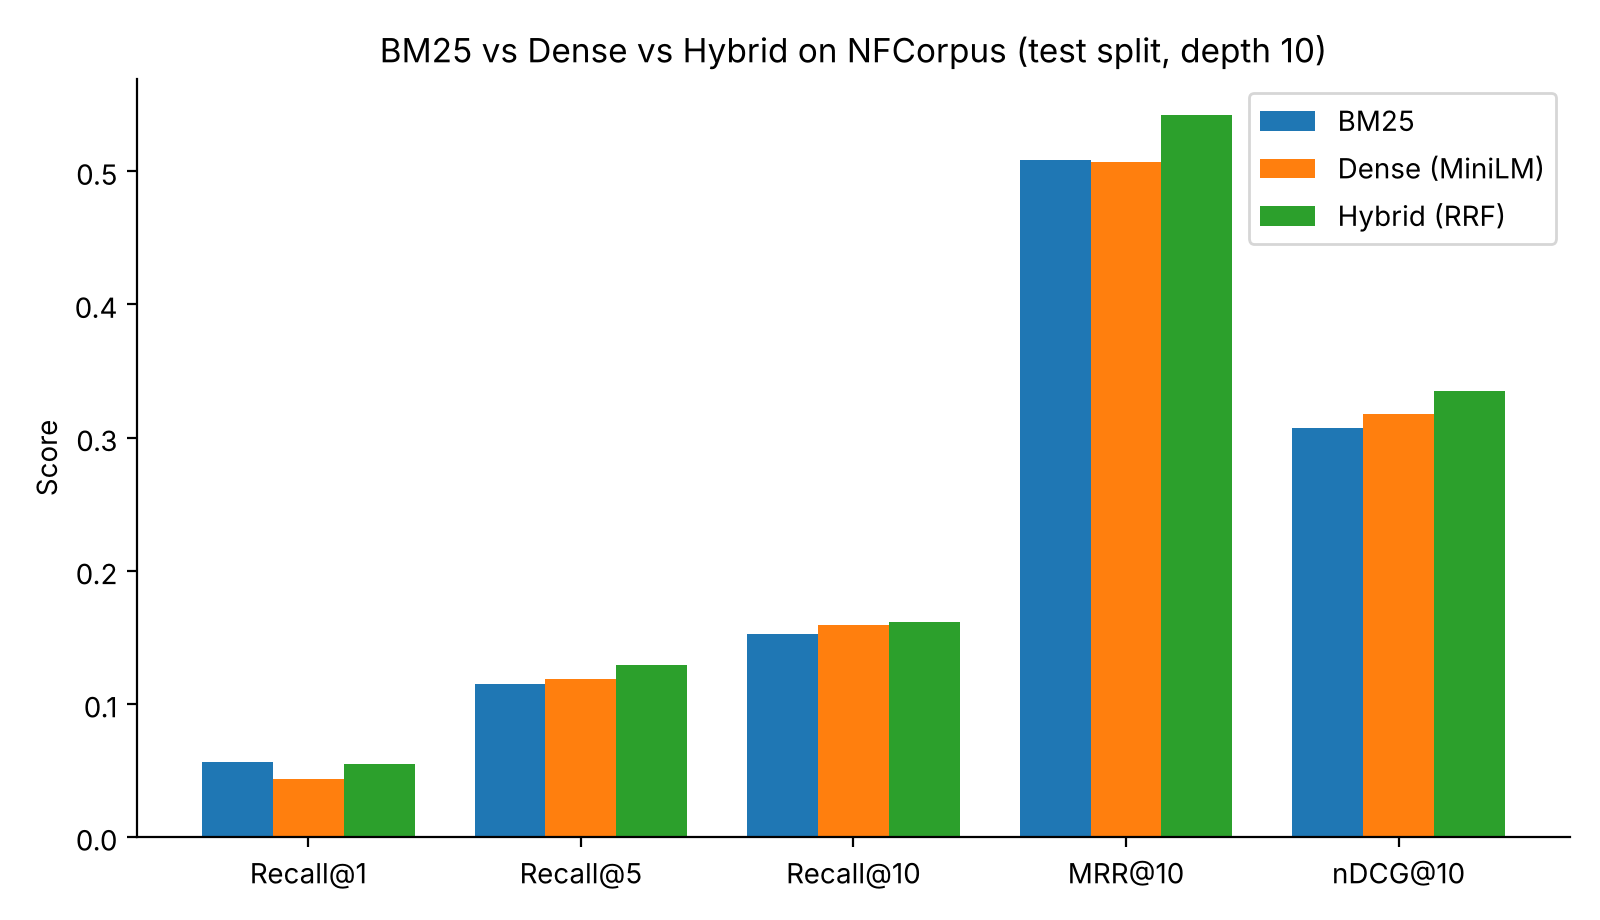
\includegraphics[width=\columnwidth]{retrieval_comparison_matched.png}
\caption{Retrieval performance by metric for all three systems (depth 10).}
\end{figure}

\textbf{Hybrid vs.\ the single methods.} Hybrid (RRF) has the highest score on four of five metrics. Relative to BM25 it improves Recall@5 by 12.4\%, MRR@10 by 6.6\% and nDCG@10 by 9.1\%; relative to dense retrieval it improves MRR@10 by 7.0\% and nDCG@10 by 5.4\%. The paired tests show that the gains over BM25 on Recall@5, MRR@10 and nDCG@10 are statistically reliable (uncorrected $p\le0.004$; nDCG@10 has $p=0.0002$), and the Recall@10 gain is marginal ($p=0.049$). Against dense retrieval, hybrid is reliably better on Recall@1, MRR@10 and nDCG@10 ($p\le0.027$) but not on Recall@5 or Recall@10. On Recall@1, hybrid and BM25 are indistinguishable ($p=0.79$).

\textbf{BM25 vs.\ dense retrieval.} Neither dominates. Dense is nominally ahead on Recall@5, Recall@10 and nDCG@10, and BM25 on MRR@10 (0.5085 vs.\ 0.5068), but none of these differences is distinguishable from zero ($p\ge0.33$). The one reliable difference is Recall@1, where BM25 is better by 0.013 ($p=0.012$). The ordering flipping with the cutoff is consistent with the two capturing different signals, the condition under which fusion is expected to help.

\begin{table*}[t]
\centering
\footnotesize
\setlength{\tabcolsep}{4pt}
\caption{Paired bootstrap tests over queries (10,000 resamples). $\Delta$ is the mean per-query difference (first system minus second); $p$ is two-sided and \emph{uncorrected}; $^\dagger$ marks $p<0.0033$ (Bonferroni threshold for 15 tests).}
\begin{tabular}{l rrr rrr rrr}
\toprule
 & \multicolumn{3}{c}{Hybrid $-$ BM25} & \multicolumn{3}{c}{Hybrid $-$ Dense} & \multicolumn{3}{c}{Dense $-$ BM25} \\
\cmidrule(lr){2-4}\cmidrule(lr){5-7}\cmidrule(lr){8-10}
Metric & $\Delta$ & 95\% CI & $p$ & $\Delta$ & 95\% CI & $p$ & $\Delta$ & 95\% CI & $p$ \\
\midrule
Recall@1  & $-$0.0014 & [$-$0.0091, 0.0042] & 0.789 & +0.0115 & [0.0033, 0.0221] & 0.0006$^\dagger$ & $-$0.0129 & [$-$0.0256, $-$0.0024] & 0.012 \\
Recall@5  & +0.0143 & [0.0046, 0.0252] & 0.0034 & +0.0106 & [$-$0.0034, 0.0252] & 0.134 & +0.0037 & [$-$0.0137, 0.0210] & 0.660 \\
Recall@10 & +0.0088 & [0.0001, 0.0186] & 0.049 & +0.0023 & [$-$0.0096, 0.0146] & 0.722 & +0.0065 & [$-$0.0089, 0.0222] & 0.397 \\
MRR@10    & +0.0337 & [0.0104, 0.0578] & 0.0036 & +0.0354 & [0.0064, 0.0640] & 0.018 & $-$0.0017 & [$-$0.0374, 0.0347] & 0.931 \\
nDCG@10   & +0.0280 & [0.0151, 0.0414] & 0.0002$^\dagger$ & +0.0170 & [0.0018, 0.0324] & 0.027 & +0.0109 & [$-$0.0109, 0.0327] & 0.326 \\
\bottomrule
\end{tabular}
\end{table*}

\subsection{Why Recall@$k$ Looks Low but MRR Is High}
Recall@$k$ values between 0.04 and 0.16 may look poor next to MRR@10 values above 0.50, but this is largely a structural property of NFCorpus. With 38.2 relevant documents per query on average, a top-10 list can contain at most 10 of them, so Recall@10 is capped at roughly $10/38.2\approx0.26$ for a typical query (the exact ceiling depends on the per-query distribution of relevant-set sizes), and Recall@1 at only a few percent. MRR, by contrast, only asks how early the \emph{first} relevant document appears, and by that measure all three systems do well. Read together, the metrics show that the systems reliably find some relevant document quickly but cannot, at a cutoff of 10, recover most of a large relevant set.

\subsection{Error Analysis: The Lexical-Overlap Mechanism}
Table~3 breaks queries down by winner.

\begin{table}[t]
\centering
\footnotesize
\setlength{\tabcolsep}{4pt}
\caption{Per-query winner (by reciprocal rank) and mean lexical overlap.}
\begin{tabular}{lccc}
\toprule
Winner & Count & \% queries & Mean overlap (SD) \\
\midrule
BM25 (higher RR)  & 73  & 22.6 & 0.303 (0.189) \\
Dense (higher RR) & 101 & 31.3 & 0.196 (0.163) \\
Tie               & 149 & 46.1 & 0.264 (0.261) \\
\bottomrule
\end{tabular}
\end{table}

Queries on which BM25 wins have a mean lexical overlap of 0.303, about 55\% higher than the 0.196 of queries on which dense retrieval wins. The difference of 0.107 is significant under a permutation test ($p=0.0001$ with the $+1$ correction; none of 10,000 shuffles produced a gap as large), its 95\% bootstrap CI is $[0.056,0.161]$, and Welch's $t$-test agrees ($t=3.92$, $p=0.00014$) with a medium effect size (Cohen's $d=0.62$). The distributions also differ at the upper end: the highest overlap among dense-win queries is 0.62, whereas BM25-win queries reach 1.00. BM25's advantage is therefore concentrated on queries that reuse the words of their relevant documents, while dense retrieval's is concentrated on queries that must be matched by paraphrase or topic. Ties (46.1\% of queries) have intermediate overlap and the widest spread.

\begin{figure}[t]
\centering
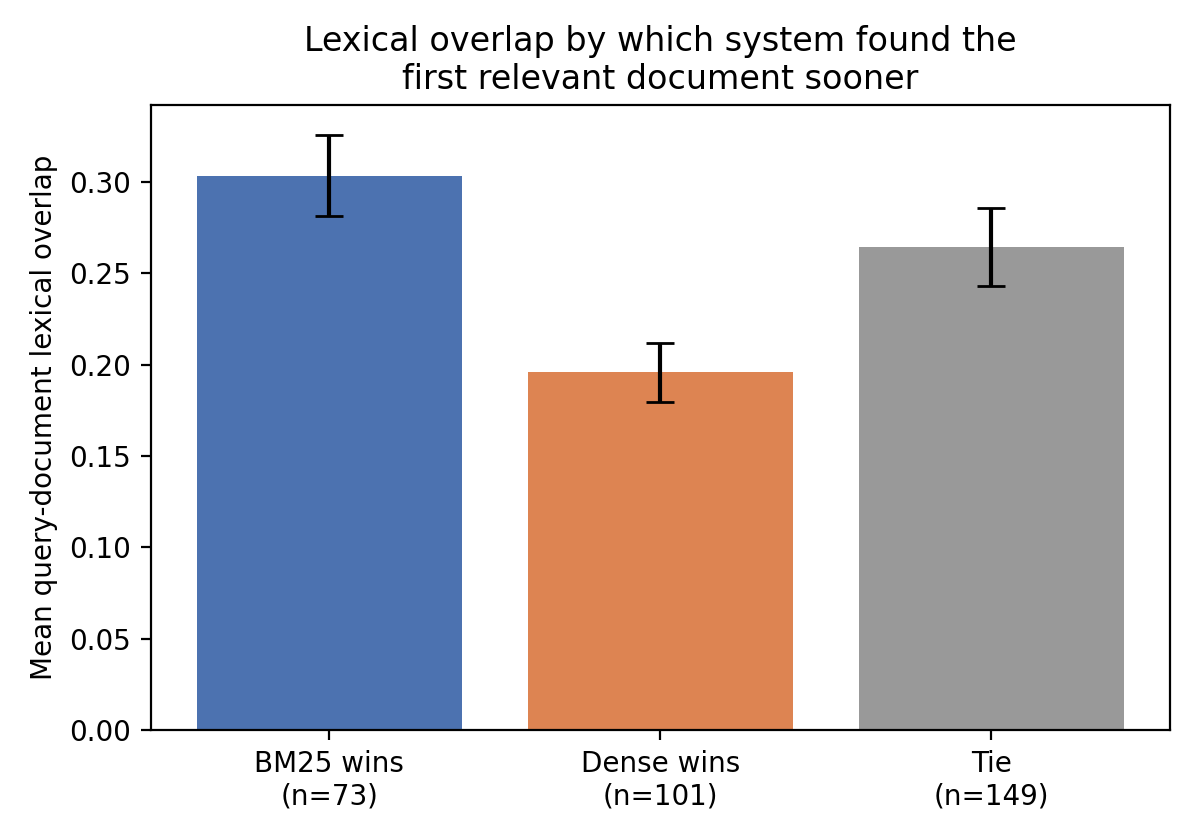
\includegraphics[width=0.92\columnwidth]{lexical_overlap_by_winner.png}
\caption{Mean lexical overlap (with standard error) by which system found the first relevant document sooner.}
\end{figure}

\subsection{Qualitative Examples}
The queries with the largest gaps in each direction are instructive (they are selected extremes, not a representative sample). Dense retrieval found no relevant document in its top 100 for the single-keyword queries ``molasses'' and ``rickets'', on which BM25 ranked a relevant document first, and was nearly as poor on ``ultra-processed foods'' and ``kohlrabi'' (reciprocal rank 0.013--0.014). Conversely, BM25 found no relevant document in its top 100 for three of the four largest dense wins (``prenatal vitamins'' and ``Apthous Ulcer Mystery Solved'', both with overlap $0.00$, and the paraphrase-style ``Preventing Cataracts with Diet''), and only at rank 11 for ``low-carb diets''. These cases fit the mechanism, but also show it is not purely lexical: several large BM25 wins have low overlap (0.17--0.33), consistent with short queries built around one rare term, where an encoder's pooled representation may dilute the key word.

One plausible reading of BM25's lead on Recall@1 is that exact-keyword matches are most likely to be placed at rank 1, whereas dense and hybrid retrieval gain at ranks 5--10 by also surfacing paraphrase-matched documents. The Recall@1 deficit of dense retrieval relative to BM25 is statistically reliable (uncorrected $p=0.012$), but the mechanism itself was not tested directly.

\subsection{Limitations}
\textbf{Correlational analysis.} Lexical overlap is only a proxy for a query reusing its answer's vocabulary. The winner label depends on the rank of the first relevant document, whereas overlap is averaged over \emph{all} relevant documents, and overlap counts stop-words, inflating it for question-style queries.

\textbf{Multiple comparisons and effect sizes.} The 15 paired tests are uncorrected. At a Bonferroni threshold of 0.0033 only hybrid over BM25 on nDCG@10 ($p=0.0002$) and hybrid over dense on Recall@1 ($p=0.0006$) survive; hybrid over BM25 on Recall@5 ($p=0.0034$) and MRR@10 ($p=0.0036$) are borderline, and Recall@10 ($p=0.049$) would not survive. Absolute gains are small.

\textbf{Single dataset, encoder and fusion rule.} Only NFCorpus, one small general-purpose encoder (all-MiniLM-L6-v2, not trained on biomedical text and truncating inputs to 256 word pieces, so long abstracts are only partially encoded), RRF with $c=60$, a regex tokenizer without stemming and untuned BM25 were used. Absolute nDCG@10 values should not be compared directly with published BEIR leaderboards, which use different BM25 implementations. Results come from one run on the standard test split.

%=====================================================================
\section{Real-World and Social Impact}
\subsection{Potential Applications}
The lexical-overlap finding is relevant to anyone deploying retrieval in a specialised domain. Where queries frequently reuse exact domain terminology (drug names, statute numbers, ticker symbols), BM25 remains a strong, cheap and interpretable baseline rather than a legacy method; the financial-QA result of \citet{akarsu2026} is consistent with this. Conversely, systems serving lay users, who describe their need in everyday language, should expect dense retrieval to carry more of the weight, and the biomedical result of \citet{bal2026} is a reminder that hybrid fusion does not always beat a good dense retriever.

For practitioners without resources for a full ablation, the results suggest a lightweight heuristic: sample a handful of representative queries, measure their lexical overlap with their expected answers, and treat high average overlap as a signal that BM25 (or a BM25-heavy hybrid) will be competitive and low overlap as a signal to invest in dense or hybrid retrieval. This is a heuristic supported by one dataset, not a guarantee. The results also argue against defaulting to dense-only retrieval without comparison: a zero-training-cost BM25 baseline came within about 6\% of the best system on Recall@10 and MRR@10, within 8\% on nDCG@10 and 11\% on Recall@5, and had the highest Recall@1 (statistically indistinguishable from hybrid).

\subsection{Fairness and Ethical Considerations}
Several fairness and ethical concerns arise in this work.

\textbf{Dataset bias:} NFCorpus is derived from PubMed abstracts and health-focused queries reflecting English-language biomedical literature. A retriever evaluated here may not generalise to other languages, health systems or lay terminology outside this register.

\textbf{Deployment risk in health contexts:} Because the queries concern medical and nutrition claims, a system built on these findings could be deployed for health-information search. Retrieval failures here (surfacing a superficially related but substantively wrong abstract) carry higher real-world cost than in general web search, so any deployment should pair strong recall with clear provenance and citation of retrieved sources rather than presenting retrieved content as verified fact.

\textbf{Reproducibility and interpretability:} Every component used (BM25, MiniLM, RRF) is open, inspectable and reproducible on commodity hardware, a meaningful property in regulated or safety-sensitive settings where an unexplainable ranking decision is itself a liability.

\textbf{AI disclosure:} This project was completed with assistance from Claude for code development, analysis and writing support.

%=====================================================================
\section{Conclusion and Future Work}
\subsection{Summary of Findings}
This paper presented a controlled three-way comparison of BM25, dense and hybrid (RRF) retrieval on NFCorpus, with three principal findings.

First, neither BM25 nor dense retrieval dominates: they are statistically indistinguishable on Recall@5, Recall@10, MRR@10 and nDCG@10, and BM25 is reliably better only on Recall@1.

Second, hybrid RRF fusion, with no tunable weight and no training, achieves the best Recall@5, Recall@10, MRR@10 and nDCG@10. Its gains over BM25 on Recall@5, MRR@10 and nDCG@10, and over dense retrieval on Recall@1, MRR@10 and nDCG@10, are reliable before multiple-comparison correction, although absolute gains are small and only a few survive a Bonferroni correction.

Third, the complementarity is associated with a measurable per-query property: queries where BM25 outranks dense retrieval have about 55\% higher query--document lexical overlap than queries where dense retrieval wins (0.303 vs.\ 0.196; permutation $p=0.0001$, Welch $p=0.00014$, Cohen's $d=0.62$, 95\% bootstrap CI $[0.056,0.161]$), a statistically supported mechanism rather than a post-hoc narrative.

\subsection{Lessons Learned}
The most important lesson is that an aggregate metric should be decomposed before it is trusted: asking \emph{why} hybrid retrieval helps produced a specific, testable answer (lexical overlap) instead of an appeal to ``combining strengths''. Low-looking absolute values (Recall@10 $\approx0.16$) can be a mechanical consequence of a dataset property (38.2 relevant documents per query) that only becomes visible next to a metric with a different structure (MRR).

Evaluation protocols must also be matched across systems: scoring BM25 and dense MRR at depth 100 but hybrid at depth 10 made the single methods look marginally better (0.5113/0.5121 vs.\ 0.5085/0.5068) and flipped their order; matched-depth scoring removed the artefact. Finally, reproducibility matters: an early version of the overlap analysis chose one relevant document per query from an unordered set, and the group gap varied between runs (0.103 in one, 0.139 in another). The effect was significant in both, but only the deterministic version yields reportable numbers.

\subsection{Future Work}
Several directions follow. Replication on further BEIR datasets such as SciFact, whose query style and vocabulary differ, would test whether the lexical-overlap relationship generalises. A weighted score-combination hybrid tuned on a validation split, and stronger or biomedical-domain encoders with stemmed, stop-word-filtered BM25, would show how much improvement remains beyond rank-only fusion with a small general-purpose model. An overlap measure that excludes stop-words and uses the first relevant document would match how the winner label is defined, and corrected or pre-registered tests would tighten the statistical claims.

\section{Acknowledgments}
The dataset was obtained through ir\_datasets and the BEIR distribution, and the encoder from the Hugging Face Hub. For feedback, email me at aadityadalal4@gmail.com

%=====================================================================
\begin{thebibliography}{9}
\bibitem[Akarsu, Karaman, and Mierbach(2026)]{akarsu2026}
Akarsu, M.; Karaman, R.~K.; and Mierbach, C. 2026.
From BM25 to Corrective RAG: Benchmarking Retrieval Strategies for Text-and-Table Documents.
\emph{arXiv preprint} arXiv:2604.01733.

\bibitem[Bal and Puhan(2026)]{bal2026}
Bal, D.~P.; and Puhan, S. 2026.
Benchmarking Retrieval Strategies for Biomedical Retrieval-Augmented Generation: A Controlled Empirical Study.
\emph{arXiv preprint} arXiv:2605.02520.

\bibitem[Boteva et~al.(2016)]{boteva2016}
Boteva, V.; Gholipour, D.; Sokolov, A.; and Riezler, S. 2016.
A Full-Text Learning to Rank Dataset for Medical Information Retrieval.
In \emph{European Conference on Information Retrieval}, 716--722.

\bibitem[Cormack, Clarke, and Buettcher(2009)]{cormack2009}
Cormack, G.~V.; Clarke, C.~L.~A.; and Buettcher, S. 2009.
Reciprocal Rank Fusion Outperforms Condorcet and Individual Rank Learning Methods.
In \emph{Proceedings of the 32nd International ACM SIGIR Conference}, 758--759.

\bibitem[Karpukhin et~al.(2020)]{karpukhin2020}
Karpukhin, V.; Oguz, B.; Min, S.; Lewis, P.; Wu, L.; Edunov, S.; Chen, D.; and Yih, W. 2020.
Dense Passage Retrieval for Open-Domain Question Answering.
In \emph{Proceedings of the 2020 Conference on Empirical Methods in Natural Language Processing}, 6769--6781.

\bibitem[Reimers and Gurevych(2019)]{reimers2019}
Reimers, N.; and Gurevych, I. 2019.
Sentence-BERT: Sentence Embeddings using Siamese BERT-Networks.
\emph{Proceedings of the 2019 Conference on Empirical Methods in Natural Language Processing}.

\bibitem[Robertson and Zaragoza(2009)]{robertson2009}
Robertson, S.; and Zaragoza, H. 2009.
The Probabilistic Relevance Framework: BM25 and Beyond.
\emph{Foundations and Trends in Information Retrieval}, 3(4): 333--389.

\bibitem[Thakur et~al.(2021)]{thakur2021}
Thakur, N.; Reimers, N.; R{\"u}ckl{\'e}, A.; Srivastava, A.; and Gurevych, I. 2021.
BEIR: A Heterogeneous Benchmark for Zero-shot Evaluation of Information Retrieval Models.
In \emph{Thirty-fifth Conference on Neural Information Processing Systems, Datasets and Benchmarks Track}.
\end{thebibliography}
\end{document}
